\section{The problem, for a reader who has never seen a tokamak}
\label{sec:physics}

This section explains the physics the benchmark is built on. A plasma physicist
can skip it; nothing later depends on more than is written here.

\subsection{What is being computed, and why anyone wants it fast}

A tokamak confines a hot plasma inside a doughnut-shaped magnetic field. For
the plasma to sit still rather than drift into the wall, the outward pressure of
the gas has to be balanced everywhere by the inward force of the magnetic field.
A configuration in which that balance holds is called an \emph{equilibrium}, and
finding it is the first thing anyone does when designing a device, planning a
discharge, or controlling one in real time.

Because a tokamak is (to a very good approximation) symmetric about its central
axis, the three-dimensional problem collapses to two dimensions: a single
cross-sectional slice, with coordinates $\Rgrid$ measured outward from the axis
of symmetry and $\Zgrid$ measured vertically. On that slice the force balance
becomes one elliptic partial differential equation, the \GS{}
equation~\citep{grad1958hydromagnetic,shafranov1958magnetohydrodynamical}:
\begin{equation}
  \Delta^{*}\psi \;=\; -\mu_{0}R^{2}p'(\psi) \;-\; F(\psi)F'(\psi),
  \qquad
  \Delta^{*} \;\equiv\;
  \frac{\partial^{2}}{\partial R^{2}}
  - \frac{1}{R}\frac{\partial}{\partial R}
  + \frac{\partial^{2}}{\partial Z^{2}} .
  \label{eq:gs}
\end{equation}

The unknown $\psi(R,Z)$ is the \emph{poloidal flux function}, measured in
webers. Two facts about it are all that the rest of this paper needs.

\textbf{The contours of $\psi$ are the surfaces the plasma lives on.} Magnetic
field lines lie within surfaces of constant $\psi$, so a plot of $\psi$ is a
picture of the magnetic structure: a set of nested closed loops around a central
peak. Figure~\ref{fig:primer}(b) is a real solution. The outermost closed
contour is the plasma boundary, conventionally the \emph{last closed flux
surface} or \lcfs{}.

\textbf{Outside that boundary, $\psi$ is not defined here.} We solve the
\emph{fixed-boundary} problem: the boundary shape is prescribed, and the
equation is solved on the region inside it. There simply is no value at grid
points outside, and the solver returns \texttt{NaN} there. About 80\% of the
grid is \texttt{NaN} in a typical case. This sounds like a bookkeeping detail.
It is the single most consequential convention in the benchmark, and
Section~\ref{sec:verification} is largely about what agents do with it.

\paragraph{Why a surrogate model is worth having.}
A finite-element \GS{} solve takes seconds. That is fine once, and ruinous
inside a loop. Device design searches over shapes; scenario planning sweeps over
operating points; real-time shape control needs an equilibrium every
millisecond, and the iterative solve is precisely the latency bottleneck that
prevents higher-bandwidth control. Learning a fast approximation of the
solver --- a \emph{surrogate} --- is therefore an active line of work in its own
right, with recent efforts targeting millisecond-scale neural-operator
equilibria~\citep{krastev2026millisecond} and control-oriented surrogates
validated on an operating device~\citep{grandin2026experimental}. The task we
set the agents is a scaled-down version of a problem people are actually paid to
solve.

\subsection{The five numbers that define a case}

The boundary is a D-shape, the standard cross-section of a modern tokamak,
described by four geometric parameters plus the current flowing in the plasma
(Figure~\ref{fig:primer}(a)):

\begin{center}
\footnotesize
\begin{tabular}{@{}llll@{}}
\toprule
\textbf{Symbol} & \textbf{Name} & \textbf{Range} & \textbf{What it does} \\
\midrule
$\rzero$  & major radius   & $0.35$--$0.55$\,m & how far the doughnut's centre sits from the axis \\
$a$       & minor radius   & $0.10$--$0.20$\,m & how fat the doughnut is \\
$\kappa$  & elongation     & $1.0$--$1.6$      & vertical stretch; $1$ is a circle \\
$\delta$  & triangularity  & $0.0$--$0.4$      & pulls the top and bottom inward into a D \\
$\Ip$     & plasma current & $80$--$200$\,kA   & sets the overall magnitude of $\psi$ \\
\bottomrule
\end{tabular}
\end{center}

\noindent Figure~\ref{fig:primer}(c) shows what the two shape parameters do.
The task, then, is to learn the map
\begin{equation}
  (\rzero, a, \kappa, \delta, \Ip) \;\longmapsto\; \psi(R,Z)
  \in \mathbb{R}^{96\times64},
\end{equation}
from a budget of solver calls the agent itself chooses.

\begin{figure}[t]
\centering
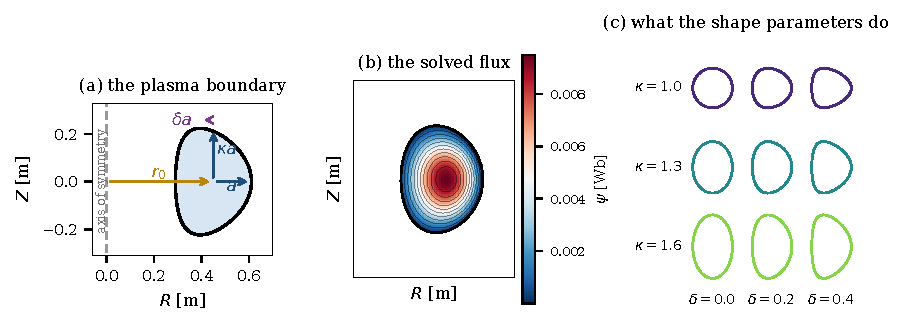
\includegraphics[width=\textwidth]{figures/fig_primer}
\caption{\textbf{(a)} The plasma boundary and the four shape parameters that set
it; the fifth, the plasma current $\Ip$, scales the field rather than the shape.
\textbf{(b)} A real solution from the frozen test set. Colour is the poloidal
flux $\psi$; the black contours are flux surfaces, and the heavy line is the
plasma boundary. Outside it, $\psi$ is undefined and the solver returns
\texttt{NaN} --- roughly 80\% of the grid. \textbf{(c)} What elongation and
triangularity do to the boundary: $\kappa$ stretches it vertically, $\delta$
pulls the top and bottom inward.}
\label{fig:primer}
\end{figure}

\subsection{How good is a prediction? Reading the error metric}

Predictions are scored by relative $L_2$ error, computed per case over the grid
points where the truth is defined:
\begin{equation}
  \relltwo_i \;=\;
  \frac{\bigl\lVert \hat{\psi}_i - \psi_i \bigr\rVert_2}
       {\bigl\lVert \psi_i \bigr\rVert_2},
  \qquad
  \text{over } \{(\Rgrid,\Zgrid) : \psi_i(\Rgrid,\Zgrid) \text{ finite}\}.
  \label{eq:rell2}
\end{equation}
Zero is perfect. The number that gives it meaning is what you get for free: a
predictor that ignores its input entirely and always returns the average flux
map of the training set scores $0.4933$ on our test set. We call that the
\emph{mean-map baseline} and quote accuracy against it,
$100\times(1 - \relltwo/0.4933)$, so that $0\%$ means ``no better than not
trying'' and $100\%$ means exact.

Because an error metric is easier to trust once you have seen it,
Figure~\ref{fig:errorcal} shows the same equilibrium predicted at a range of
\relltwo{} values by actual runs from our campaign. Below about $0.1$ the
prediction is visually indistinguishable from the truth. By $0.2$ the field is
noticeably blurred. At the mean-map baseline it is a smear with no case-specific
structure at all, and beyond that the predictor is contributing nothing.

\begin{figure}[t]
\centering
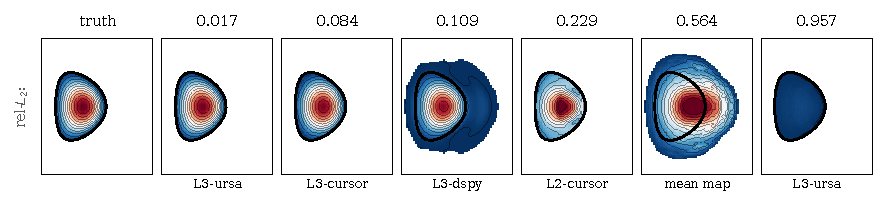
\includegraphics[width=\textwidth]{figures/fig_error_calibration}
\caption{What the error metric looks like. The same test equilibrium, predicted
by six actual runs spanning the range we observed, with \relltwo{} for that case
above each panel and the condition that produced it below. ``Mean map'' is the
input-independent baseline. All panels share a colour scale.}
\label{fig:errorcal}
\end{figure}
